\chapter{Packages}
\label{ch:package}
\newenvironment{packclass}[0]{\textbf{Contained classes:} \begin{itemize}
}{\end{itemize}}
\newenvironment{packenum}[0]{\textbf{Contained enums:} \begin{itemize}
}{\end{itemize}}
\newenvironment{packif}[0]{\textbf{Contained interfaces:} \begin{itemize}
}{\end{itemize}}
\newenvironment{packpack}[0]{\textbf{Contained packages:} \begin{itemize}
}{\end{itemize}}
\newcommand{\packobj}[1]{\item #1}
\newcommand{\abstract}[1]{\textit{abstract} #1}

In this chapter, all packages and their purpose are introduced.

\section{MORR}

\begin{center}
    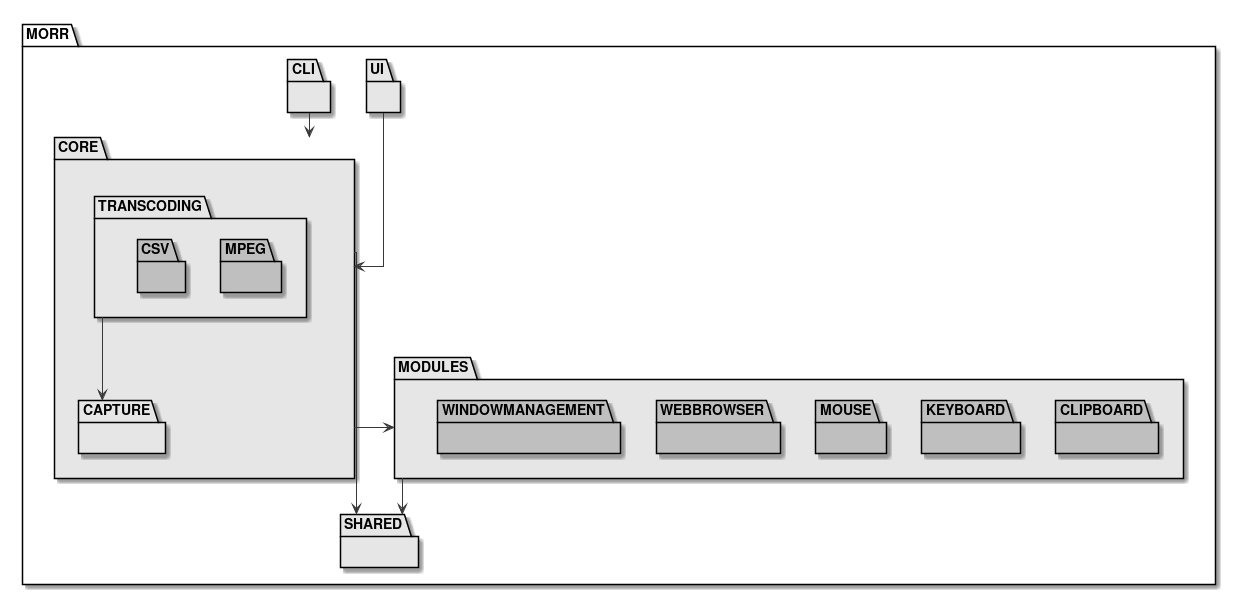
\includegraphics[width=1.0\textwidth]{resources/Packages/AllPackages.png}
\end{center}

The MORR package is the master package containing the whole application. It does not contain any classes directly as it only serves as a container for all packages required in the design.

\newpage
\section{MORR.CORE}

\begin{center}
    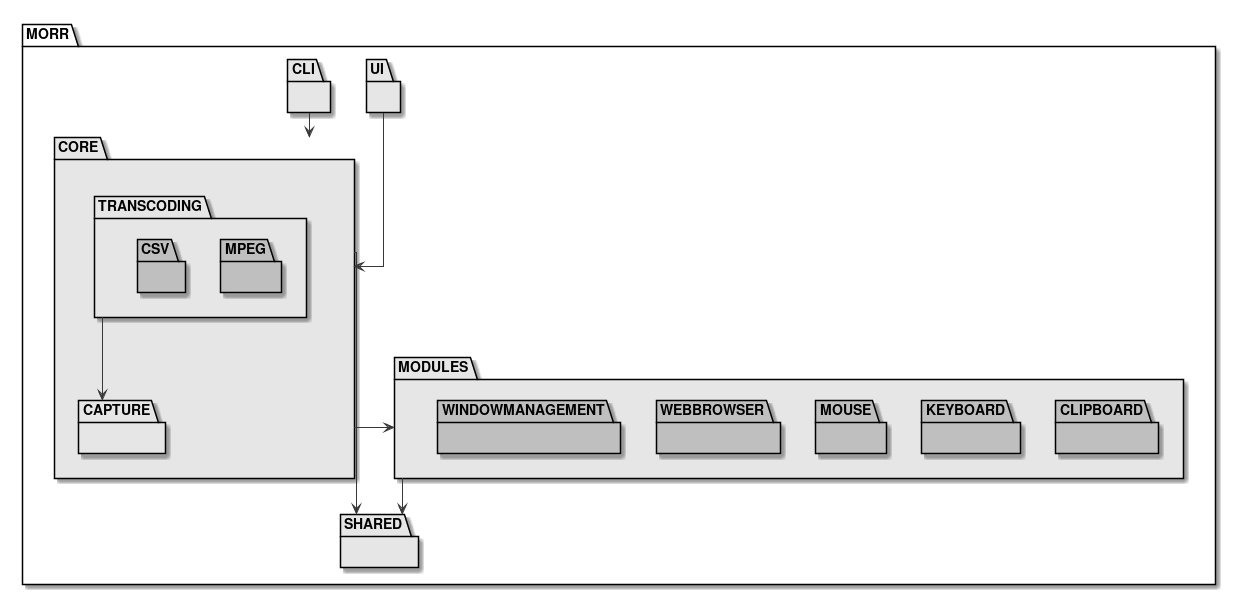
\includegraphics[width=1.0\textwidth]{resources/Packages/AllPackages.png}
\end{center}

The \textbf{CORE} package contains the central initializing logic to be called when the program is started and coordinates state-changes while the application is running.

\begin{packclass}
\packobj{RecordingManager}
\packobj{Bootstrapper}
\packobj{ModuleManager}
\packobj{ConfigurationManager}
\end{packclass}

\begin{packif}
\packobj{IModuleManager}
\packobj{IBootstrapper}
\packobj{IConfigurationManager}
\packobj{IRecordingsManager}
\end{packif}

\newpage
\section{MORR.CLI}

\begin{center}
    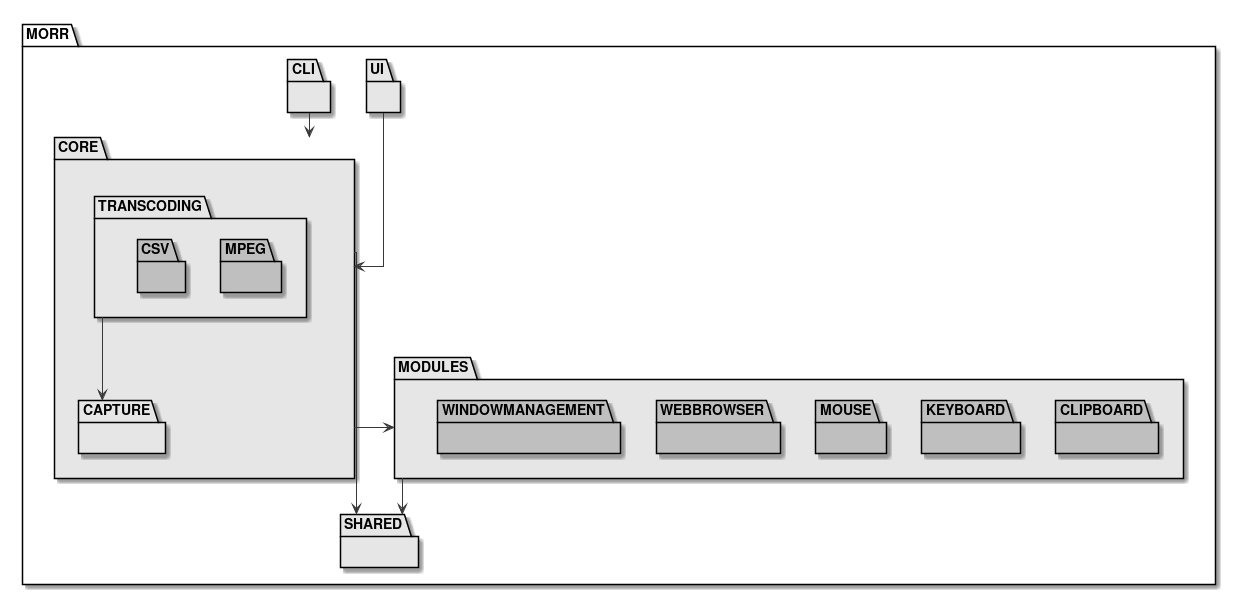
\includegraphics[width=1.0\textwidth]{resources/Packages/AllPackages.png}
\end{center}

The \textbf{CLI} package contains all logic exclusively needed for the command line interface which allows for the extraction of event data from saved recordings.

\begin{packclass}
\packobj{ProcessCommand}
\packobj{Executor}
\packobj{OutputFormatter}
\packobj{Options}
\packobj{Program}
\end{packclass}

\newpage
\section{MORR.SHARED}

\begin{center}
    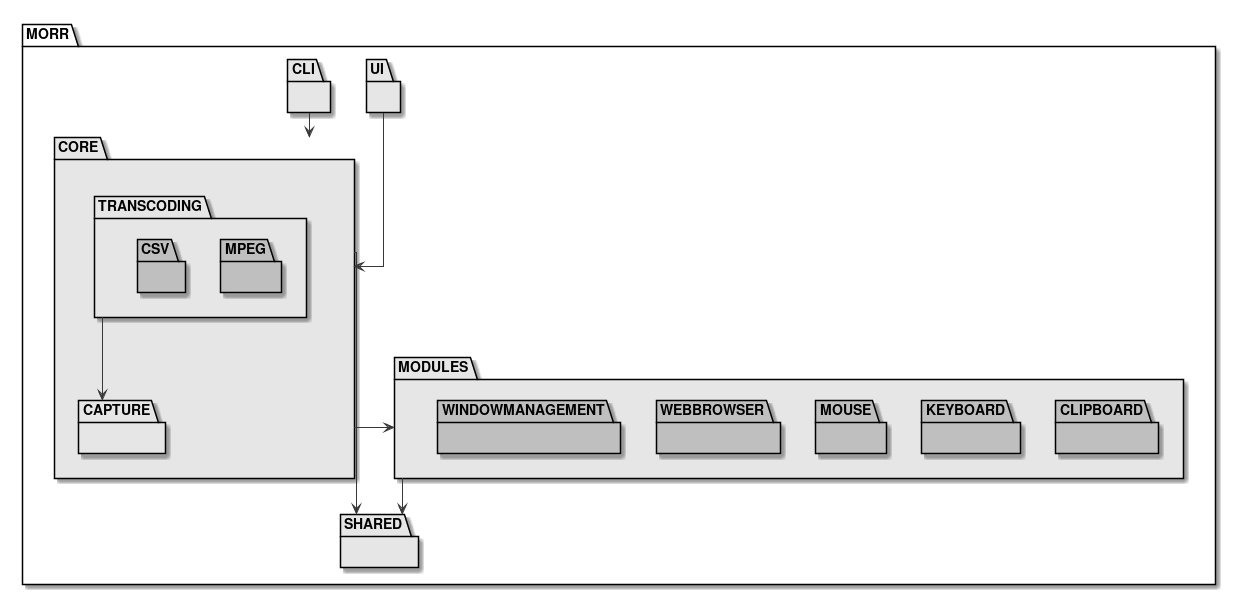
\includegraphics[width=1.0\textwidth]{resources/Packages/AllPackages.png}
\end{center}

The \textbf{SHARED} package provides interfaces and classes which have to be known and shared across multiple packages, such as the concept of an event or a module.

\begin{packif}
\packobj{IConfiguration}
\packobj{IModule}
\packobj{ITransformingModule}
\packobj{ICollectingModule}
\packobj{IReceivingModule}
\packobj{IReadOnlyEventQueue<out T>}
\packobj{IEventQueueStorageStrategy}
\end{packif}

\begin{packclass}
\packobj{\abstract{EventQueue<T>}}
\packobj{\abstract{Event}}
\packobj{InvalidConfigurationException}
\packobj{RingBufferStorageStrategy<T>}
\packobj{RefCountedListStorageStrategy<T>}
\packobj{KeepAllStorageStrategy<T>}
\end{packclass}

\newpage
\section{MORR.TRANSCODING}

\begin{center}
    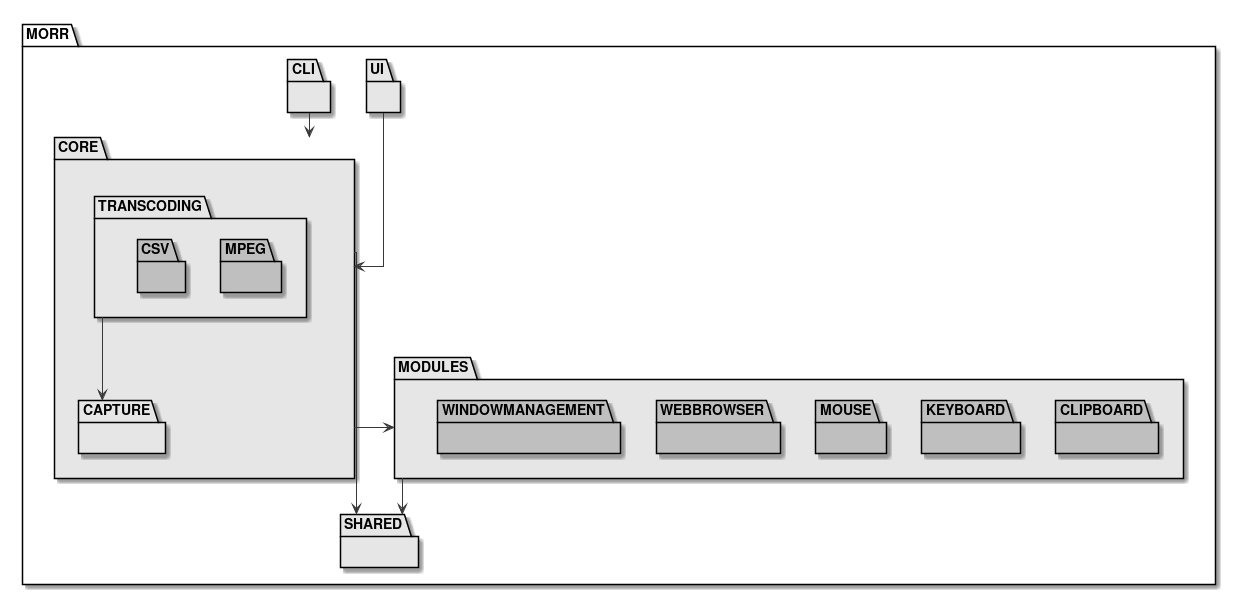
\includegraphics[width=1.0\textwidth]{resources/Packages/AllPackages.png}
\end{center}

The \textbf{TRANSCODING} package is responsible for serialization and deserialization of recorded video-, audio- and event-data. 

Contained interfaces:
\begin{itemize}
\item IVideoCapture
\item IAudioCapture
\item IDecoder
\item IEncoder
\end{itemize}

Contained classes:
\begin{itemize}
\item \textit{abstract} AudioSample
\item \textit{abstract} VideoSample
\item \textit{abstract} MetadataSample
\item DecodingException
\item EncodingException
\item CaptureException
\item MetadataDecodingException
\item AudioDecodingException
\item VideoDecodingException
\item MetadataEncodingException
\item AudioEncodingException
\item VideoEncodingException
\item VideoCaptureException
\item AudioCaptureException
\end{itemize}

Contained packages:
\begin{itemize}
\item CSV
\item MPEG
\end{itemize}

\section*{MORR.TRANSCODING.CSV}
The \textbf{TRANSCODING.CSV} package is responsible for providing functionality which allows for encoding/decoding events from/to CSV (comma separated values) format.

Contained classes:
\begin{itemize}
\item CSVDecoder
\item CSVEncoder
\end{itemize}

\section*{MORR.TRANSCODING.MPEG}
The \textbf{TRANSCODING.MPEG} package allows for storing video-, audio- and event-data in a MPEG container and also retrieving this data again from such a container.

Contained classes:
\begin{itemize}
\item CSVDecoder
\item CSVEncoder
\end{itemize}

\newpage
\section{MORR.MODULES}

\begin{center}
    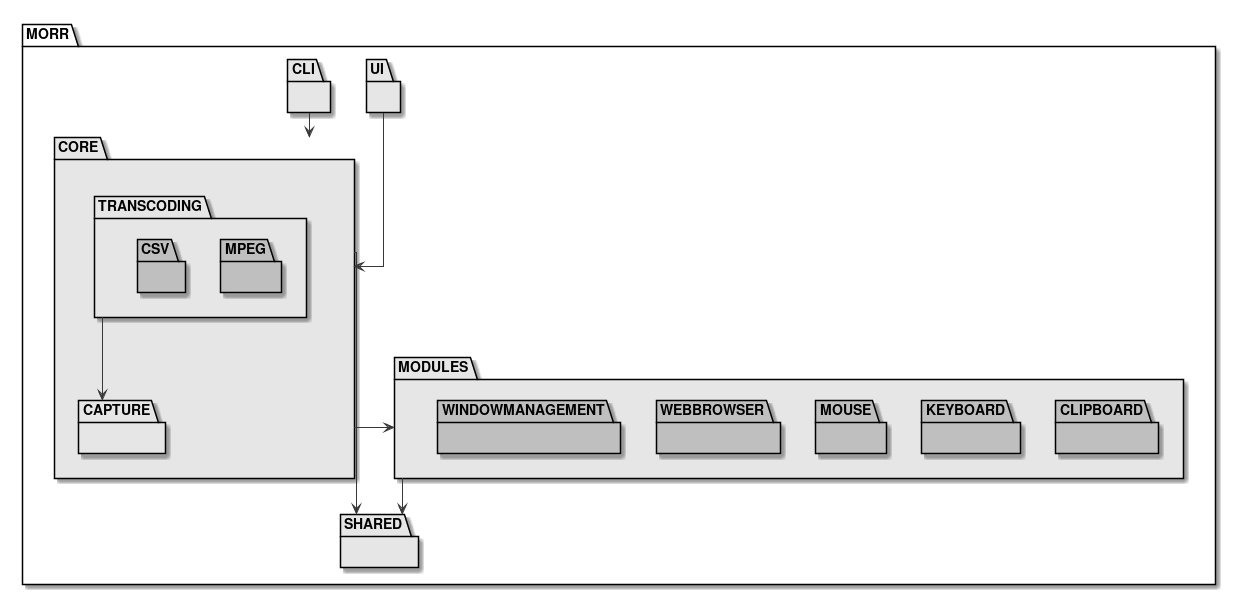
\includegraphics[width=1.0\textwidth]{resources/Packages/AllPackages.png}
\end{center}

The \textbf{MODULES} package serves as a container for all module-subpackages.

\subsection*{MORR.MODULES.WINDOWMANAGEMENT}

\begin{center}
    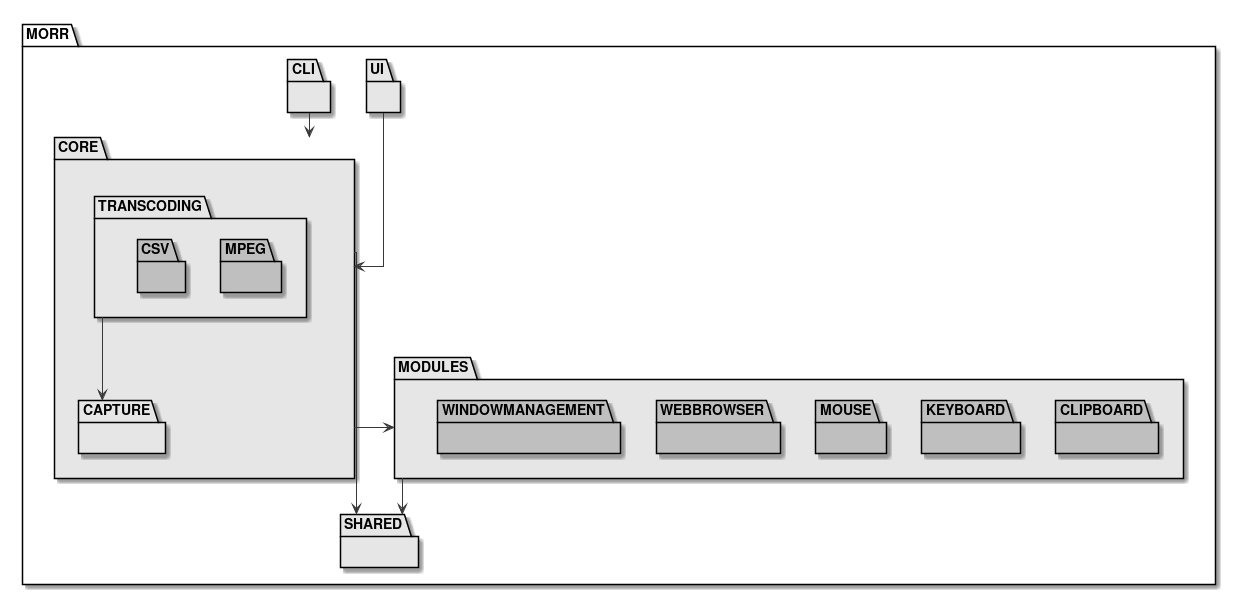
\includegraphics[width=1.0\textwidth]{resources/Packages/AllPackages.png}
\end{center}

The \textbf{WINDOWMANAGEMENT} package is responsible for providing the classes and concepts necessary for recording the window related user-interactions.

Contained classes:
\begin{itemize}
\item WindowManagementModule
\item \textit{abstract} WindowEvent
\item WindowMovementEvent
\item WindowFocusEvent
\item WindowSateChangedEvent
\item WindowResizingEvent
\end{itemize}
\newpage
\subsection*{MORR.MODULES.KEYBOARD}

\begin{center}
    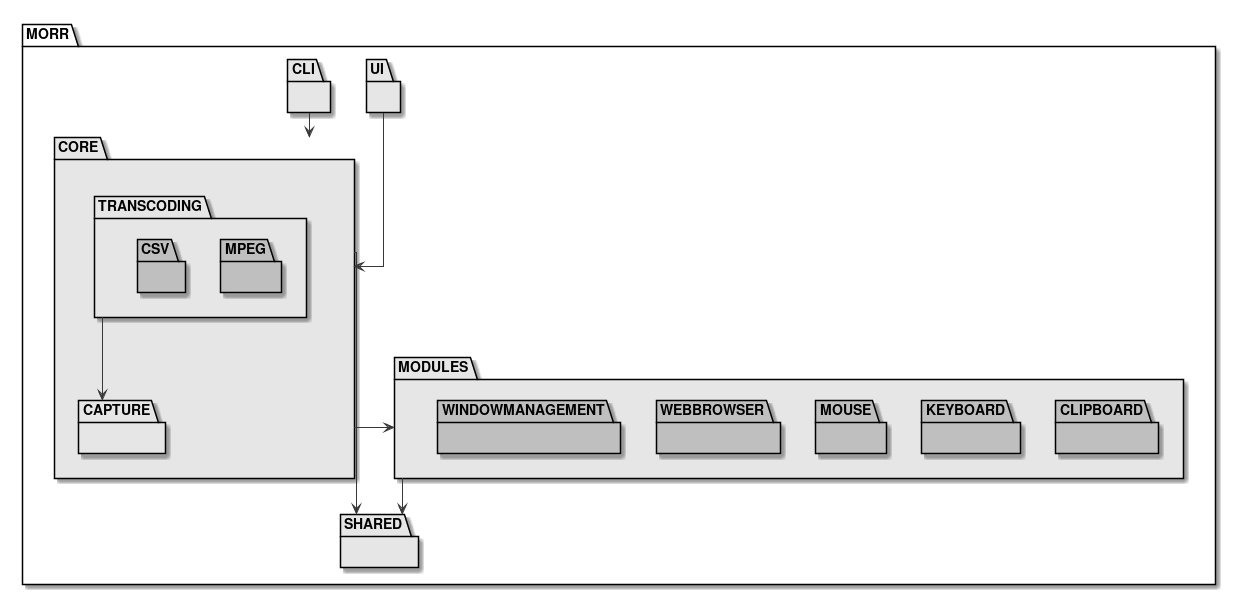
\includegraphics[width=1.0\textwidth]{resources/Packages/AllPackages.png}
\end{center}

The \textbf{KEYBOARD} package is responsible for providing the classes and concepts necessary for recording the keyboard related user-inputs.

Contained classes:
\begin{itemize}
\item \textit{abstract} KeyboardEvent
\item KeyboardModule
\item KeyboardInteractEvent
\end{itemize}

\newpage
\subsection*{MORR.MODULES.WEBBROWSER}

\begin{center}
    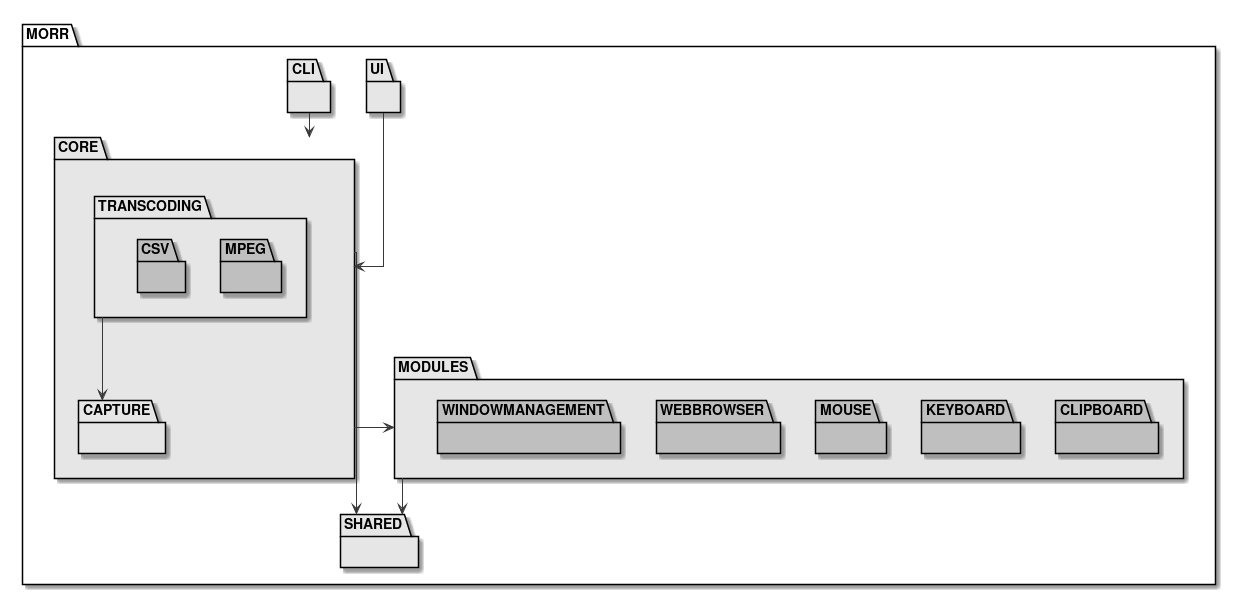
\includegraphics[width=1.0\textwidth]{resources/Packages/AllPackages.png}
\end{center}

The \textbf{WEBBROWSER} package is responsible for providing the classes and concepts necessary for recording the webbrowser related user-interactions.

Contained classes:
\begin{itemize}
\item WebBrowserModule
\item \textit{abstract} WebBrowserEvent
\item TextSelectionEvent
\item TextInputEvent
\item SwitchTabEvent
\item OpenTabEvent
\item CloseTabEvent
\item NavigationEvent
\item HoverEvent
\item FileDownloadEvent
\item ButtonClickEvent
\end{itemize}

\newpage
\subsection*{MORR.MODULES.CLIPBOARD}

\begin{center}
    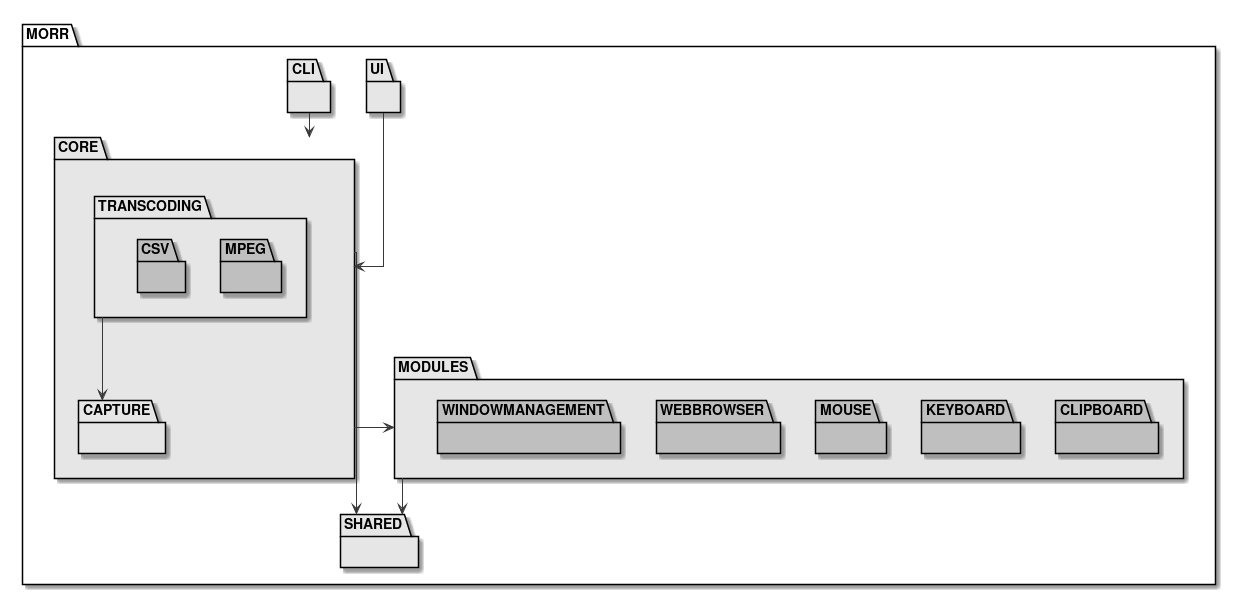
\includegraphics[width=1.0\textwidth]{resources/Packages/AllPackages.png}
\end{center}

The \textbf{CLIPBOARD} package is responsible for providing the classes and concepts necessary for recording the clipboard related user-interactions.

Contained classes:
\begin{itemize}
\item ClipboardModule
\item \textit{abstract} ClipboardEvent
\item ClipBoardInteractEvent
\end{itemize}

Contained enums:
\begin{itemize}
\item InteractionType
\end{itemize}

\newpage
\subsection*{MORR.MODULES.MOUSE}

\begin{center}
    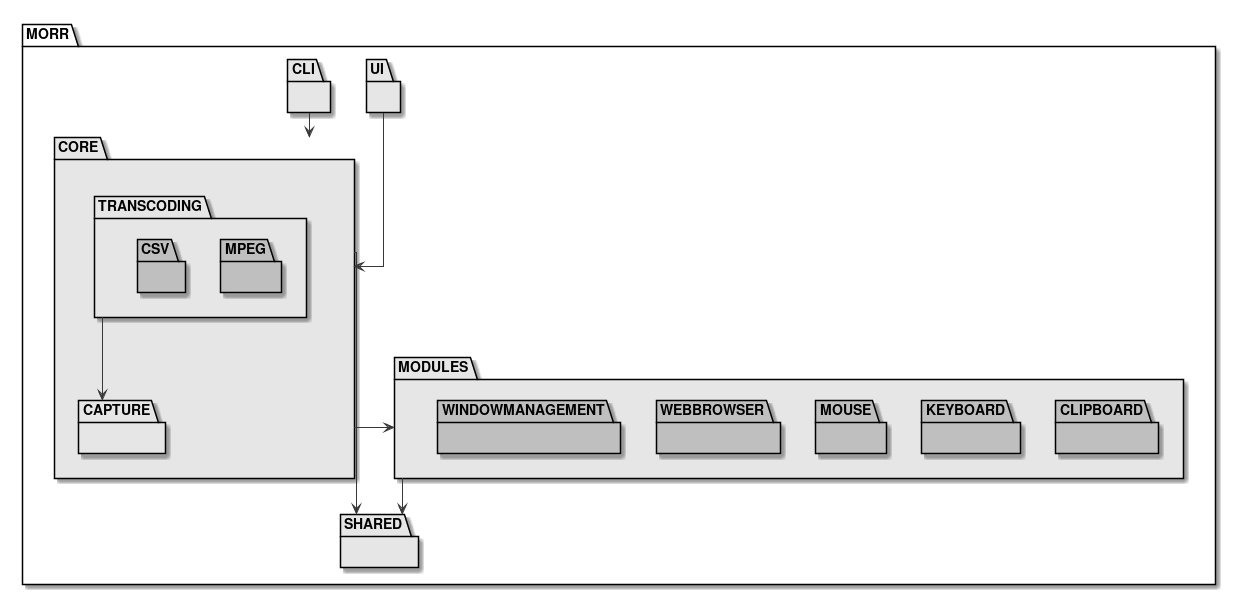
\includegraphics[width=1.0\textwidth]{resources/Packages/AllPackages.png}
\end{center}

The \textbf{MOUSE} package is responsible for providing the classes and concepts necessary for recording the mouse related user-inputs.

Contained classes:
\begin{itemize}
\item MouseModule
\item \textit{abstract} MouseEvent
\item MouseScrollEvent
\item MouseClickEvent
\item MouseMoveEvent
\end{itemize}

Contained enums:
\begin{itemize}
\item MouseButton
\item MouseButtonState
\end{itemize}
